\chapter{Theoretical Basics}

This chapter introduces the theoretical basis needed in this thesis. The first half of this chapter presents the initial knowledge of the tracking algorithm, including the general dynamic system model, Kalman filter, motion models and multitarget tracking. The important algorithms for optimization and classification are reviewed in the second half of this chapter. The optimization algorithms are explained briefly at the start of Section 2.3. Then the method of grid search and Bayesian optimization is in detail explained. In Section 2.4, the principle of SVM is explained. In the following section, overfitting and the methods for avoiding it are discussed.

\section{Single-Target Tracking}
\label{st}

% \textcolor{red}{(of course we need tracking) what is the tracking process(estimation of a dynamic system) - what is the estimation - introduce single target tracking because it's the simplest tracking system and the basis of MTT. }

% \textcolor{red}{Then in subsection: 1. the dynamic system (needed for tracking process) 2. estimation with KF(estimation) 3. motion model}


The tracking process can be recognized as a state estimation problem of a dynamic system. The simplest dynamic system in the tracking problem is the single-target tracking (STT) system that assumes only one target at the same time in the area of interest. The STT is also the basis for the multitarget tracking.

\subsection{Dynamic System Model}

A typical time-discrete dynamic system can be represented by functions between random variables. The random state vector $\boldsymbol{\underline{x}}_{t}$ is a function of the random state in the last timestep $\boldsymbol{\underline{x}}_{t-1}$, the external input $\hat{\underline{u}}_{t-1}$ and the random system noise $\boldsymbol{\underline{w}}_{t-1}$ with a given distribution \cite{welch1995introduction}.  Therefore, the state transition function $a_{t}$  can be represented with the function

\begin{equation}
    \boldsymbol{\underline{x}}_{t+1} = a_{t}(\boldsymbol{\underline{x}}_{t},\,\hat{\underline{u}}_{t},\,\boldsymbol{\underline{w}}_{t}).
\end{equation}

The measurement $\boldsymbol{\underline{z}}_{t}$ is a function of the state of the tracked object $\boldsymbol{\underline{x}}_{t}$ and the random measurement noise $\boldsymbol{\underline{v}}_{t}$ with a given distribution \cite{welch1995introduction}. Therefore, the measurement function $h_{t}$ can be represented with the function

\begin{equation}
    \boldsymbol{\underline{z}}_{t} = h_{t}(\boldsymbol{\underline{x}}_{t},\,\boldsymbol{\underline{v}}_{t}).
\end{equation}

In this thesis, the tracking problem was assumed as with a linear time-invariant (LTI) system that follows the linear state transition model. Further, the motion model and noise in the tracking process are assumed to be identical for all time steps and all objects, hence the time index of the system matrices can be neglected. The system has also no external input. Therefore, the state transition model can be represented with these two functions

\begin{gather}
    \boldsymbol{\underline{x}}_{t+1}^{\mathrm{Lin}} = \mathbf{F}\boldsymbol{\underline{x}}_{t}^{\mathrm{Lin}}+\boldsymbol{\underline{w}}\\
    \boldsymbol{\underline{z}}_{t}^{\mathrm{Lin}} = \mathbf{H}\boldsymbol{\underline{x}}_{t}^{\mathrm{Lin}}+\boldsymbol{\underline{v}}.
\end{gather}

In these two functions, the matrix $\mathbf{F}$ contains the information of the state transition model. The matrix $\mathbf{H}$ contains the information of the measurement system. The vector $\boldsymbol{\underline{w}}$ and $\boldsymbol{\underline{v}}$ represent respectively the system and measurement noise.


\subsection{Kalman Filter}
\label{kf}

Estimation is defined as the process of inferring the value of a quantity from indirect and uncertain observations. Filtering is the estimation of the state of a dynamic system from noisy observations amounts by ``filtering out" the noise \cite{bar2004estimation}. The Kalman filter is the most prevalent method for solving linear tracking problems having independent Gaussian random errors with zero mean \cite{stone2013bayesian}. It provides an efficient computational means to estimate the state of a process, in a way that minimizes the mean of the squared error between the estimation and the real state of the system  \cite{maybeck1982stochastic}. 

The Kalman filter estimates the state of a dynamic system by using a form of feedback control: the filter estimates the system state at the next timestep and then obtains feedback in the form of noisy measurements. As such, the algorithm for the Kalman filter can be divided into two parts: prediction step and update step, as depicted in Figure \ref{Structure Kalman filter}. 

\begin{figure}[htbp]
\centering
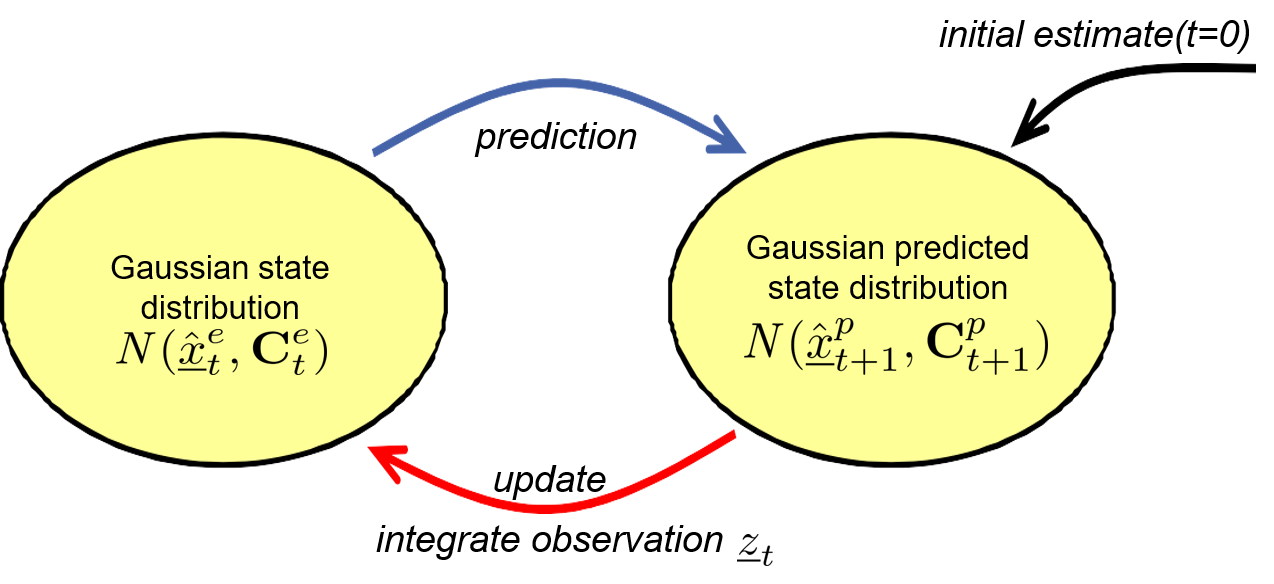
\includegraphics[width=0.8\textwidth]{figures/Structure Kalman Filter2.png}
\caption{The cycle of the recursive Kalman filter. The prediction process generates the state estimation with the estimated state from the last timestep and the given motion model. The update process updates the system state on the base of measurements  \cite{welch1995introduction}.}
\label{Structure Kalman filter}
\end{figure}

The equations in the prediction step are responsible for predicting the state $\hat{\underline{x}}^{\mathrm{p}}_{t+1}$ and the error covariance $\textbf{C}_{t+1}^{\mathrm{p}}$ to obtain the \textit{a priori} estimation for the next time step. The equations for the prediction step are presented as 
\begin{gather}
    \hat{\underline{x}}^{\mathrm{p}}_{t+1}=\mathbf{F}\hat{\underline{x}}^{\mathrm{e}}_{t}\\
    \mathbf{C}_{t+1}^{\mathrm{p}}=\mathbf{F}\mathbf{C}_{t}^{\mathrm{e}}\mathbf{F}^\top+{ \mathbf{C}_{t}^{\underline{\boldsymbol{w}}}}, 
\end{gather}

where the matrix $\mathbf{C}_{t}^{\underline{\boldsymbol{w}}}$ represents the system noise that depends on the difference between real system state transition and the predefined system model. The system matrix $\mathbf{F}$ and the system noise matrix $\mathbf{C}_{t}^{\underline{\boldsymbol{w}}}$ contains all the information about the system model required by the Kalman filter \cite{pfaff2019multitarget}.

The update equations are responsible for incorporating the new measurements with the \textit{a priori} estimation to obtain an improved \textit{a posteriori} estimation that contains the estimated state $\hat{\underline{x}}^{\mathrm{e}}_{t}$ and error covariance $\mathbf{C}_{t}^{\mathrm{e}}$. The equations for the update step are presented as
\begin{gather}
    \textbf{K}_{t}=\textbf{C}_{t}^{\mathrm{p}}\mathbf{H}({\textbf{C}_{t}^{\underline{\boldsymbol{v}}}}+\mathbf{H}\textbf{C}_{t}^{\mathrm{p}}\mathbf{H}^\top)^{-1}\\
    \textbf{C}_{t}^{\mathrm{e}}=(1-\textbf{K}_{t}\mathbf{H})\textbf{C}_{t}^{\mathrm{p}}\\
    \hat{\underline{x}}^{\mathrm{e}}_{t}=\hat{\underline{x}}^{\mathrm{p}}_{t}+\textbf{K}_{t}(\hat{\underline{z}}_{t}-\mathbf{H}\hat{\underline{x}}^{\mathrm{p}}_{t}), 
\end{gather}

where the matrix $\mathbf{H}$ contains the information of the measurement system and the matrix $\mathbf{C}_{t}^{\underline{\boldsymbol{v}}}$ represents the measurement noise that depends on the measurement accuracy. With the optimal Kalman gain $\textbf{K}_{t}$, the estimation error $\left \| \hat{\underline{x}}_{t}-\hat{\underline{x}}^{\mathrm{e}}_{t} \right \|$ is minimized \cite{welch1995introduction}.

However, the exact system and measurement covariance matrices are hard to obtain for most of the real systems. As a result, the Kalman filter often works with incorrect noise matrices. The sensitivity analysis describes the sensitivity of the estimation error to incorrectly input noise matrices in the estimator \cite{lu2014false}. In this thesis, the values of these input matrices will be the hyperparameters for the sensitivity analysis and the optimization.



\subsection{Motion and Measurement Model in Tracking}
\label{cv basic}
% \textcolor{red}{This part is changed with 1-D CV model, the 2-D case is moved to chapter 3. Title changed to "motion and measurement model"}
The motion model is the system model for the tracking problem, which describes the motion of the tracked objects in the tracking process. There are many motion models based on different system characteristics, which mainly include the position, velocity and angular velocity of tracked objects \cite{li2003survey}\cite{schubert2008comparison}. 

The constant velocity model is a widely used simple motion model for tracking. In this model, the velocity of tracked objects are considered as constant, and the accelerations are assumed to be zero in noise-free cases. However, the velocity does not remain really ``constant" in the tracking. As a part of the state vector, the value of the velocity can change because of the measurement noise.

Take the 1-D constant velocity model as an example. In the model, the state vector contains the position and velocity of the tracked objects along and vertical to the transport directions \cite{pfaff2019multitarget}
\begin{equation}
    \underline{x}_{t}=
    \begin{bmatrix}
        \mathsf{x}_{t}\\ 
        \dot{\mathsf{x}}_{t}
    \end{bmatrix}.
\end{equation}

The system matrix for the constant velocity model is
\begin{equation}
    \mathbf{F}=\begin{bmatrix}
     1 & T \\ 
     0 & 1
    \end{bmatrix} ,
\end{equation}
with $T$ denoting the time between two subsequent time steps. 

The system noise covariance is given by
\begin{equation}
    \mathbf{C}^{\underline{\boldsymbol{w}}}=S^{\boldsymbol{w}}
    \begin{bmatrix}
     T^3/3 & T^2/2\\ 
     T^2/2 & T 
    \end{bmatrix} ,
\end{equation}
where the $S^{\boldsymbol{w}}$ is the power spectral density of the system noise.

Only the position can be directly observed in the measurement process. Therefore, the measurement matrix is
\begin{equation}
    \mathbf{H}=\begin{bmatrix}
     1 & 0
    \end{bmatrix} .
\end{equation}

The measurement position variance is represented with the measurement noise power spectral density $S^{\boldsymbol{v}}$ in this case, as
\begin{equation}
    \mathbf{C}^{\underline{\boldsymbol{v}}}=S^{\boldsymbol{v}}.
\end{equation}

The real motion of the particles does not exactly follow these motion models. These inaccuracies in the motion model are included in system noise terms. With carefully selected noise terms, such as the system and measurement noise level, the system noise could represent the model inaccuracies better, and the tracking error can be therefore reduced. As stated in \Sec{kf}, these noise terms serve as the hyperparameters in the following chapters.


\FloatBarrier

% \section{Multitarget Tracking Algorithm}
% \label{mt}

% In this part, the algorithm for the multitarget tracking is in detail explained.

\section{Data Association for Multitarget Tracking}

Multitarget tracking refers to the step-by-step state estimation of multiple objects simultaneously. A fully automatic multitarget tracking algorithm needs the ability to deal with an unknown number of targets, unknown target initiation and termination times as well as false measurements \cite{musicki2009multiscan}. With the multitarget tracking algorithms, new measurements are constantly assigned to the objects, and the predictions of the object states are also generated recursively. We are provided with measurements at each timestep, and at each timestep several measurements can be observed. In this thesis, each measurement contained in the dataset is assumed as belonging to exactly one object and should therefore be assigned to it. As depicted in Figure \ref{tracking system}, the multitarget tracking algorithm includes two main parts: single-target state estimation and data association.

\begin{figure}[htbp]
\centering
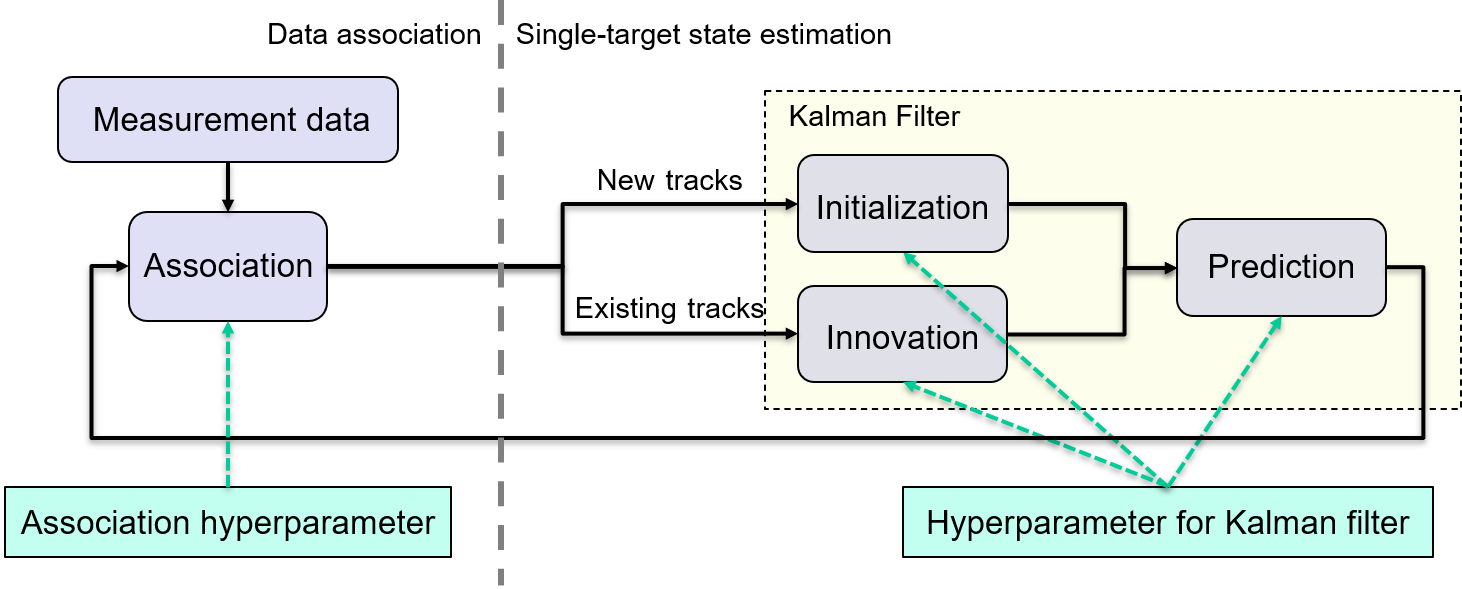
\includegraphics[width=0.9\textwidth]{figures/tracking system.png}
\caption{Structure of the multitarget tracking algorithm.}
\label{tracking system}
\end{figure}

% \subsection{Data Association}

In the tracking problem, we need to update the new state of each object with the measurement data. However, in the multitarget tracking problem the correspondence information between each measurement and object is usually not provided. Therefore, we need the data association algorithms to establish this correspondence. With the data association, each measurement is assigned to an object. Then the original multitarget tracking problem is transferred into many single-target tracking problems that are much easier to solve.

There are many types of data association algorithms. A basic idea is to assign the measurement to the object, whose predicted position is closest to the measurement. When the assignment process is done consecutively, this method is the local nearest neighbor (LNN). However, this method often leads to incorrect association decisions, as shown in Figure \ref{lnn} \cite{pfaff2019multitarget}.

\begin{figure}[htbp]
\centering
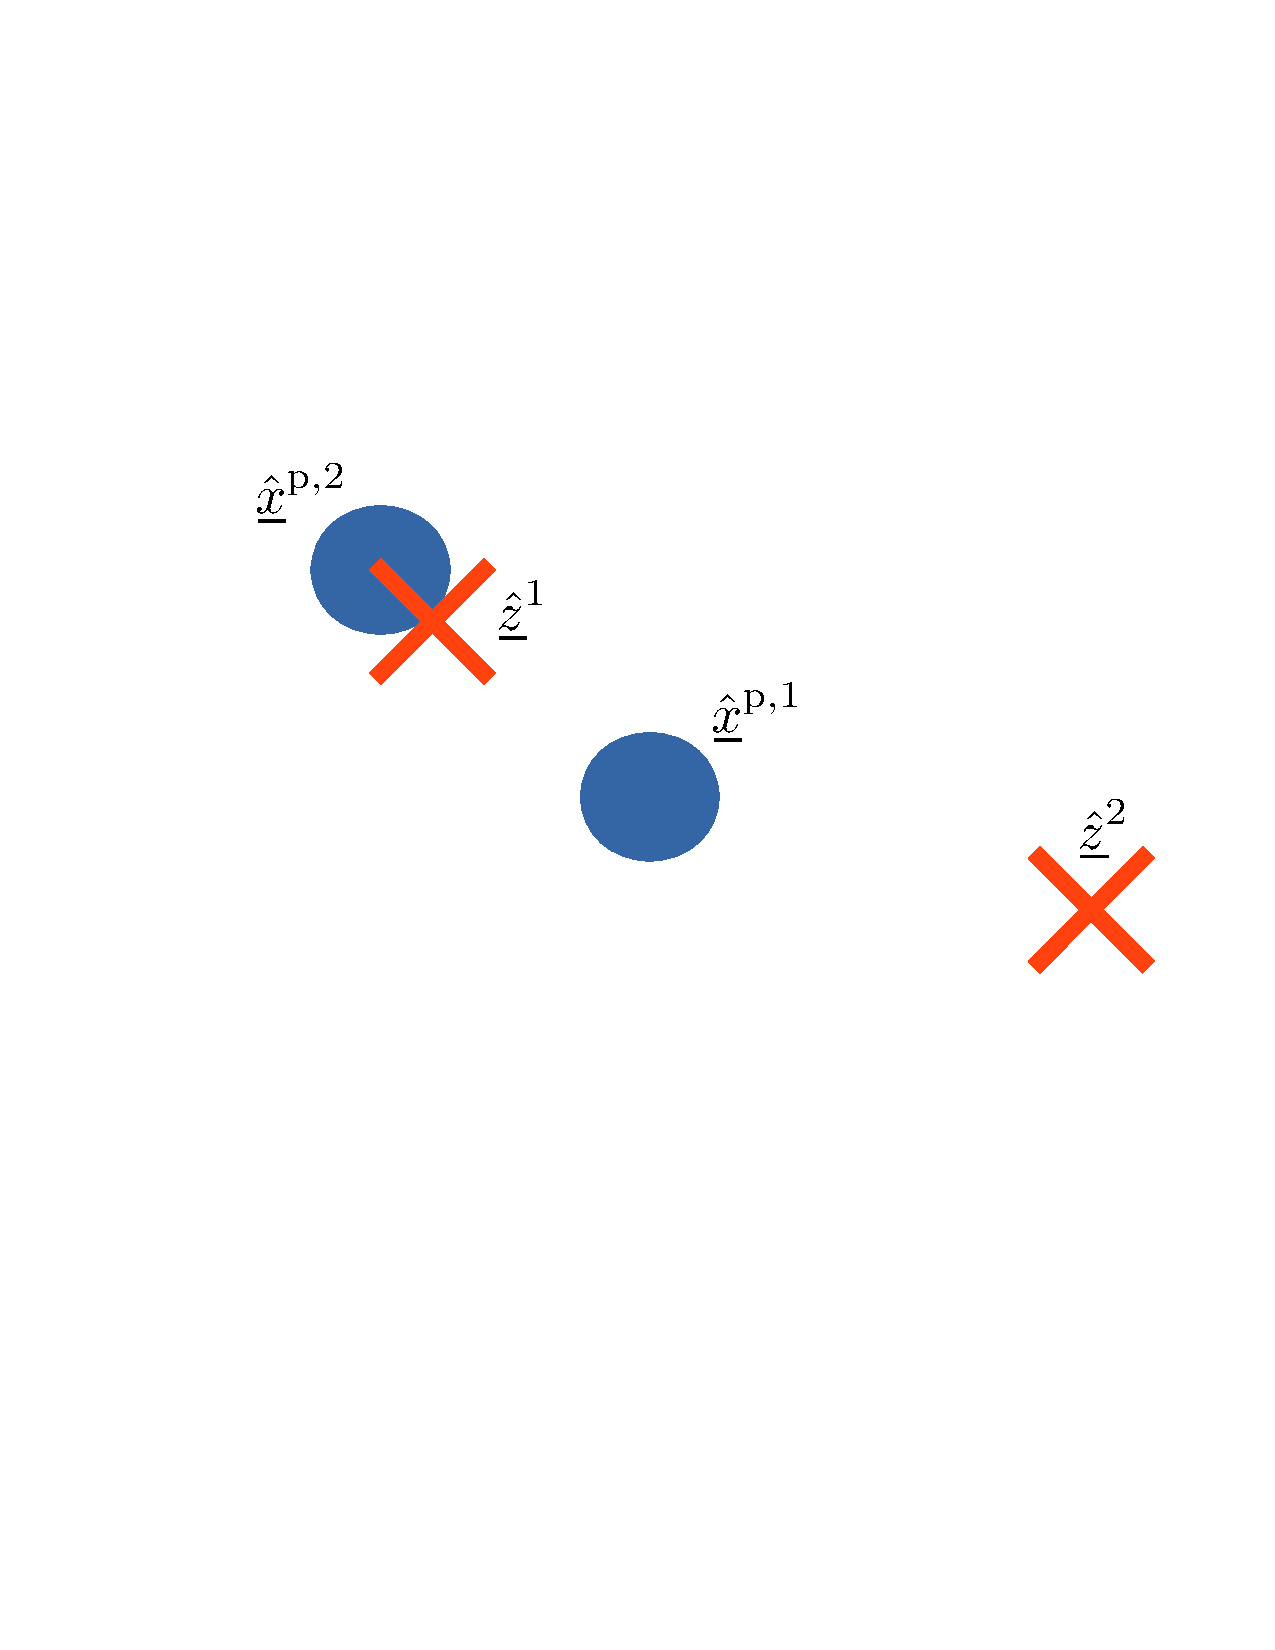
\includegraphics[width=0.5\textwidth]{figures/LNN.pdf}
\caption{Example in which the LNN may perform badly. If the $\hat{\underline{z}}^{2}$ is assigned before $\hat{\underline{z}}^{1}$, it will be assigned to $\hat{\underline{x}}^{\mathrm{p},2}$, which leads to an association error \cite{pfaff2019multitarget}.}
\label{lnn}
\end{figure}

The global nearest neighbor (GNN) optimizes the overall quality of the association decision by determining the association decision that minimizes the sum of the distances of all track–measurement pairs. 
% \textcolor{red}{I deleted the "squared Mahalanobis" here, because I think only mentioning the distance is enough for explaining the principle of GNN. The Mahalanobis is in detail explained in the next chapter.} 
The GNN has more complexity than the LNN, but it can significantly improve the accuracy of the association. Therefore, the GNN is chosen from the multitarget tracking algorithm. 
% The more detailed description of the implementation of the GNN and tracking algorithm is presented in \Sec{mt}. 

One extension of the GNN is the multi-hypotheses tracking, where the algorithm gives several hypotheses of the association in each step of the tracking process, and the update processes are also done with different hypotheses. The most possible hypothesis in the end will be chosen as the final association result \cite{blackman2004multiple}. However, multi-hypotheses tracking is not suitable for real-time tracking in the implementation used in this thesis because of the high computational costs \cite{pfaff2019multitarget}. 

Until now, we are introducing the hard association methods that were used in our implementation, where each measurement is assumed to belong to exactly one object and each state updation is based on only one measurements. However, there are also several other data association methods using the soft association, where one measurement can be used to update several tracks. There are soft association algorithms using the joint probabilistic data association \cite{fortmann1983sonar} or the Markov chain Monte Carlo based particle filter \cite{khan2005mcmc}. However, these algorithms usually have high computational requirements and are sometimes hard to integrate with other parts of the implemented multitarget tracking algorithm we are using. For these reasons, these algorithms are not considered in the multitarget tracking algorithm used in this thesis.

In some cases, the feature of the objects can also be used for the association. Algorithms using the object features have been widely used in many areas, such as tracking of humans in videos \cite{wu2006tracking}. Following this idea, integrating the object information into the association can be a possible extension of the tracking algorithm.

% \subsection{State Update and Estimation}

% \textcolor{red}{still necessary here?}
% In the last part, the multitarget tracking problem is transferred into many single-target tracking problems. Therefore, a Kalman filter with a selected motion model is used for solving these problems. The Kalman filter updates the state prediction for each track, which is used for the data association of the next timestep. 

% The algorithm for this part is more detailed explained in \Sec{st}. 

\FloatBarrier

\section{Optimization Algorithms}

% \textcolor{red}{Added a very short introduction of the objective functions}
Optimization is the minimization or maximization of an objective function subject to constraints on its variables \cite{nocedal2006numerical}. There are many algorithms proposed for optimization, which can be mainly divided into two classes. One is the gradient-based optimization that computes the gradient of the loss function of the hyperparameters and then optimizes the hyperparameters using gradient descent. However, many systems are too complicated to have the explicated solution for the gradient of the loss function, which limits the application of the gradient-based optimization only on some specific problems, such as hyperparameter optimization in support vector machines \cite{chapelle2002choosing} or logistic regression \cite{foo2008efficient}. 

The other optimization methods, such as grid search, random search, Bayesian optimization and evolutionary algorithms need no gradient information of the loss function. These methods treat the system for optimization as a black box. In grid search, the main algorithm computes the loss function with a tuple of hyperparameters from the predefined parameter space in each search and selects the best hyperparameter set minimizing the loss function. Bayesian optimization creates a surrogate model from the observed value of the loss function replacing the original loss function, and determine the optimized point based on the surrogate model. Evolutionary optimization makes numerous observations in each step and breeds the observation point for the next timestep from the observation with lower losses. These methods have different features and are used in different scenarios \cite{claesen2015hyperparameter}\cite{feurer2019hyperparameter}.

% A hyperparameter is a parameter of a learning algorithm that is set prior to training and remains constant during training.

\subsection{Objective Function}

The objective function evaluates the performance of a model or an algorithm on the given data. An objective function is either a loss function to be minimized, or a reward function that needs to be maximized. For example, the prediction error introduced in \Sec{loss function} is the loss function for our optimization.

Given a function $f(x,y)$, there can be two types of objective function with the difference of the optimizing object. The first type is to find the maximum or minimum of the function, as $\max f(x,y)$. The other type is to find the values of some variables within the constraints that minimize (or maximize) the objective function, for example, $\underset{x\in \mathbb R,\ y\in \mathbb R}{\arg \max }\ f(x,y)$. In general, we are more interested in the second type of object function.


There are different objective functions for different optimization problems. The functions always depend on the optimization objection. There are two important types of problems in machine learning: regression and classification. In regression, a model is trained for mapping the input variables to continuous output variables that fit the observations \cite{balasubramanian2014conformal}. Therefore, the mean squared error (MSE) $(\sum _{i=1}^{n}(y_{i}-{\hat {y_{i}}})^{2})/n$ and the mean absolute error (MAE) $(\sum_{i=1}^{n} \left | y_{i}-\hat{y_{i}} \right |)/n$, which show the distance between the observations and predictions, are the most common objective functions. In the expression, the $y_{i}$ and $\hat{y_{i}}$ means respectively the $i$th observed and predicted value, and the $n$ indicates the number of predictions. 

The classification problem needs to approximate a mapping function (f) from input variables to discrete output variables. Therefore, the MSE and MAE can be also used in the classification problem for evaluating the difference between the predicted and observed classes. There are also some common loss functions only for discrete classes, such as the cross-entropy loss $-\sum_x p(x)log\,q(x)$, where the $p$ and $q$ indicates observed and predicted probability distribution.






% \textcolor{red}{But most of optimization problem like $\arg \max \ f(x,y)$ is able to obtain the $\max f(x,y)$ at the same time?}

% \textcolor{red}{To some extent the optimization of hyperparameters is also a type of regression? Find hyperparameters to build a model to fit the measurements(input) and the last measurements of tracks(output). The loss function is MAE for prediction error of each track.}
% Although there are

% \textcolor{red}{Is it all right for these math expressions stay in text or it should in a separated display?} 

% \textcolor{red}{Should I give a more detailed description of the regression problems?} 



% \textcolor{red}{And should I give a more detailed description of the classification problems? The SVM has its own loss function.} 

\subsection{Grid Search}
\label{gs}

% \textcolor{red}{define the HP}

Grid search is the most traditional and intuitive way for the optimization of hyperparameters \cite{ataei2004using}. The procedure of grid search is shown in Figure \ref{grid search}. At first, a set of sample values are determined for each hyperparameter for optimization. Then the main algorithm of grid search runs with hyperparameters in the Cartesian product of these sets, which is the so-called grid points, and evaluates the performance with the value of the objective function \cite{bergstra2012random}. 

Since the grid search algorithm returns the value of the objective function of all grid points, it is possible to evaluate the effect of different hyperparameters on the objective function, as the blue area shown in Figure \ref{grid search}. The best hyperparameter set can also be chosen as the hyperparameter set that results in the minimum error.

\begin{figure}[htb]
\centering
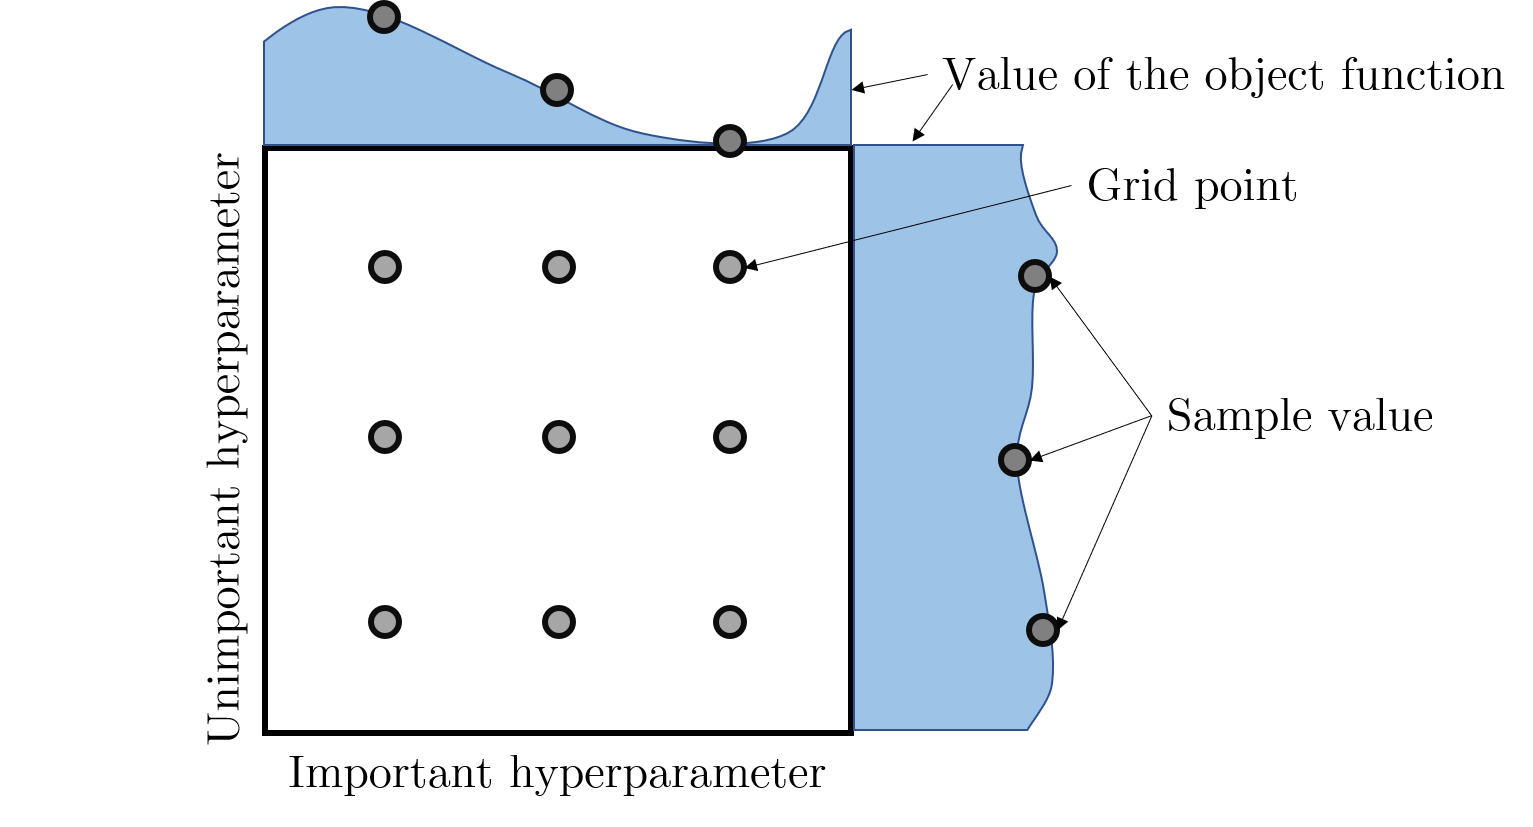
\includegraphics[width=0.8\textwidth]{figures/grid search.png}
\caption{Illustration of grid search, showing the sample points, grid points and different effects of the hyperparameters on the value of the objective function \cite{bergstra2012random}.}
\label{grid search}
\end{figure}

Grid search is easy to implement and understand, but not efficient. First, the grid points to check in grid search increases exponentially with the number of hyperparameters, thus grid search is not practical with too many hyperparameters. Second, the grid points need to be chosen manually before the optimization, which means choosing the appropriate sample values of the hyperparameter can be challenging work. Furthermore, the searches are limited in the grid points, so the final optimized point provides not necessarily the real optimal value of hyperparameters. At last, each search in grid search can be independent. It means that the selection of hyperparameters of each search can not use the information of the objective function from former searches, which is a waste of the computation power \cite{bergstra2012random}. For the reasons above, grid search is often combined with other optimization methods, which used for giving an initial impression of the effect of hyperparameters or reducing the dimension of hyperparameters for the next step of optimization \cite{ataei2004using}.

\subsection{Bayesian Optimization}
\label{bayopt intro}

% \textcolor{red}{todo: rewrite this part with less words and more equations}

Bayesian optimization is a state-of-the-art optimization framework for the global optimization of functions. Bayesian optimization only depends on the discrete observed values of the objective function, without using any gradient information of the objective function. This method is one of the most efficient approaches in terms of the number of function evaluations required. Therefore, this method suits especially the problems, where the objective function is unable to be expressed with a differentiable function or expensive to calculate \cite{brochu2010tutorial}.

\begin{figure}[htbp!]
\centering
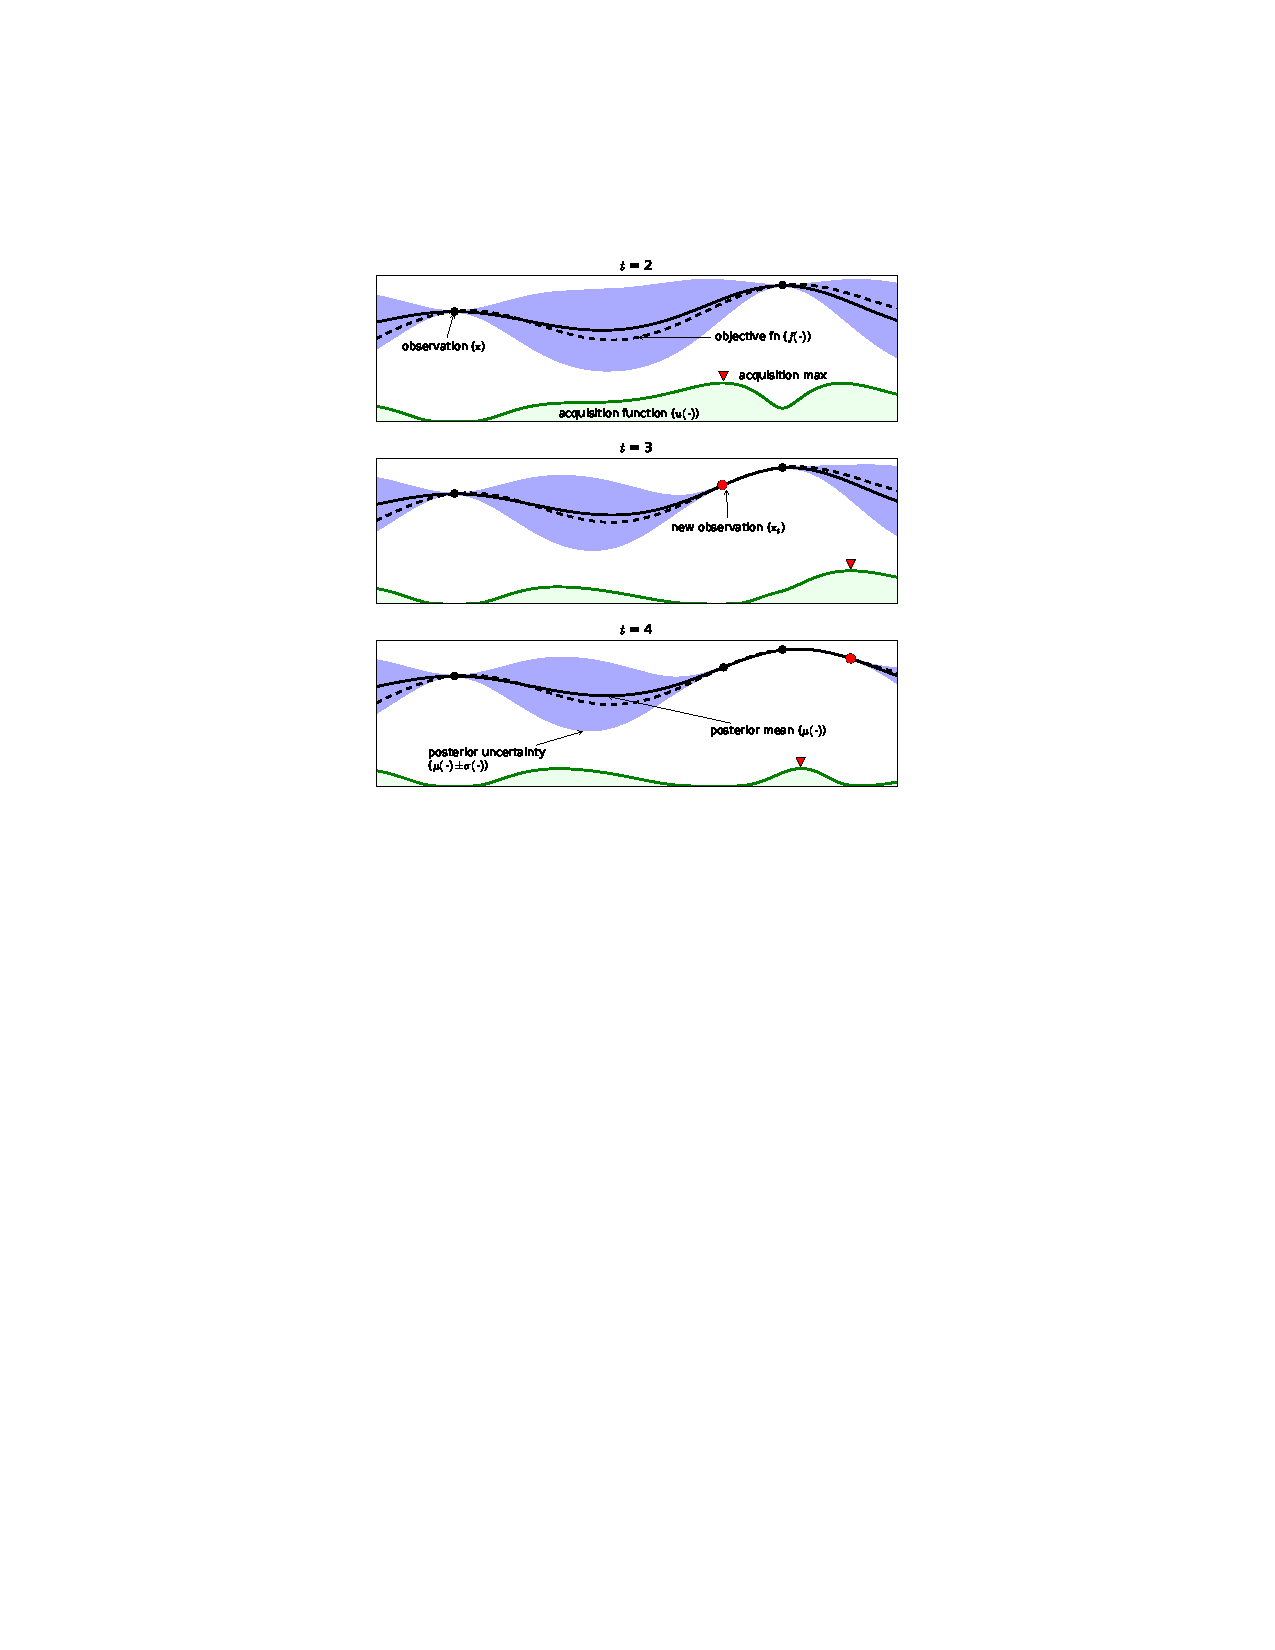
\includegraphics[width=0.8\textwidth]{figures/bay opt.pdf}
\caption{The figures demonstrate an example of Bayesian optimization. The posterior means function of the surrogate model is shown in the black solid line, and the original objective function is shown in the black dash line. After each iteration, the surrogate model is updated according to the observation result. The blue shade shows the variance of the model. The unsampled area has high uncertainty, and uncertainty at observed points is reduced to 0. The acquisition function is shown in the lower green shaded plots. When the estimated objective function or uncertainty is high, the acquisition is also high, which indicates a high possibility for the maximum of the objective function. The sample point for the next iteration is chosen from the maximum of the acquisition function, as the red triangle marks shown at $t=3$ and $t=4$ \cite{brochu2010tutorial}.}
\label{bayesian optimization}
\end{figure}


% \begin{algorithm}[!h]
% \caption{Bayesian optimization \cite{shahriari2015taking} \textcolor{red}{line number?need improve}}
% \label{Bayesian optimization algorithm}
% \begin{algorithmic}[1]
%     \FOR{$t=1,2,....$}
%         \State Select new $\mathbf{x}_{t+1}$ by optimizing acquisition function $\alpha$: \\ $\mathbf{x}_{t}=\mathop{\argmax}_{\mathbf{x}}{\alpha(\mathbf{x};\mathcal{D}_{1:t-1})}$\\
%         \State Make the observation: $y_{t}=f(\mathbf{x}_{t+1})+\varepsilon_{t}$ 
%         \Comment{Expensive step} \\
%         \State Augment data: $\mathcal{D}_{1:t}=\{\mathcal{D}_{1:t-1},(\mathbf{x}_{t},y_{t})\}$
%         \State update statistical model
%     \ENDFOR
% \end{algorithmic}
% \end{algorithm}


Bayesian optimization is an iterative algorithm that updates a probabilistic surrogate model $f(\mathbf{x})$ and an acquisition function $\alpha$ after every iteration. The surrogate model is an estimation of the objective function that is based on the value of observations of the objective function from each iteration. With this model, the algorithm can avoid estimating the original objective function, which is often too complicated. After enough iterations, the posterior mean function of the surrogate model will become similar to the objective function.

The Gaussian process (GP) prior is well-suited as the surrogate model. A GP is a random function represented with its mean function $m$ and covariance function $k$
\begin{equation}
    f(\mathbf{x}) \sim \mathcal{G} \mathcal{P}\left(m(\mathbf{x}), k\left(\mathbf{x}, \mathbf{x}^{\prime}\right)\right).
\end{equation}
This function returns the mean and variance of a normal distribution over the possible values of $f$ at $\mathbf{x}$ \cite{brochu2010tutorial}. One of the very common covariance functions is the squared exponential function
\begin{equation}
    k\left(\mathbf{x}_{i}, \mathbf{x}_{j}\right)=\exp \left(-\frac{1}{2}\left\|\mathbf{x}_{i}-\mathbf{x}_{j}\right\|^{2}\right).
\end{equation}
Given the first $t$ observation samples, we can use the Gaussian process to calculate the possible distribution of the observations using the Sherman-Morrison-Woodbury formula \cite{sherman1950adjustment}, namely
\begin{equation}
    P\left(f_{t+1} | \mathcal{D}_{1 : t}, \mathbf{x}_{t+1}\right)=\mathcal{N}\left(\mu_{t}\left(\mathbf{x}_{t+1}\right), \sigma_{t}^{2}\left(\mathbf{x}_{t+1}\right)\right),
\end{equation}
where
\begin{gather}
\mu_{t}\left(\mathbf{x}_{t+1}\right) =\mathbf{k}^{T} \mathbf{K}^{-1} \mathbf{f}_{1 : t} \\ 
\sigma_{t}^{2}\left(\mathbf{x}_{t+1}\right) =k\left(\mathbf{x}_{t+1}, \mathbf{x}_{t+1}\right)-\mathbf{k}^{T} \mathbf{K}^{-1} \mathbf{k}\\ \mathbf{K}=\left[\begin{array}{ccc}{k\left(\mathbf{x}_{1}, \mathbf{x}_{1}\right)} & {\dots} & {k\left(\mathbf{x}_{1}, \mathbf{x}_{t}\right)} \\ {\vdots} & {\ddots} & {\vdots} \\ {k\left(\mathbf{x}_{t}, \mathbf{x}_{1}\right)} & {\dots} & {k\left(\mathbf{x}_{t}, \mathbf{x}_{t}\right)}\end{array}\right].
\end{gather}

The acquisition function guides the selection of the sample point for the next iteration step, using the predicted distribution of the surrogate model. The acquisition function is designed for showing the potential maximum of the objective function, where the prediction or the uncertainty is high. There are many different criteria for the computation of the acquisition function. The probability of improvement acquisition function maximizes the probability of the value of objective function higher than the observed maximum objective value, as
\begin{equation}
    \mathrm{PI}(\mathbf{x}) =P\left(f(\mathbf{x}) \geq f\left(\mathbf{x}^{+}\right)+\xi\right),
\end{equation}
where $\mathbf{x}^{+}$ denotes the maximum value observed in former timesteps and $\xi$ indicates a trade-off parameter controlling the exploration and exploitation. When $\xi$ is high, the algorithm would have more tendency of exploration.

The expected improvement acquisition function maximizes the expected improvement with respect to $f(\mathbf{x}^{+})$. The expected improvement function is defined as
\begin{align} 
\centering
\mathrm{EI}(\mathbf{x}) &=\left\{\begin{array}{ll}{\left(\mu(\mathbf{x})-f\left(\mathbf{x}^{+}\right)-\xi\right) \Phi(Z)+\sigma(\mathbf{x}) \phi(Z)} & {\text { if } \sigma(\mathbf{x})>0} \\ 
{0} & {\text { if } \sigma(\mathbf{x})=0}\end{array}\right.\\, \end{align}
\begin{equation}
    Z =\frac{\mu(\mathbf{x})-f\left(\mathbf{x}^{+}\right)-\xi}{\sigma(\mathbf{x})} ,
\end{equation}
where $\phi(\cdot)$ and $\Phi(\cdot)$ denote respectively the PDF and CDF. $\xi$ is still a trade-off parameter for controlling the exploration and exploitation here.

The computation of the acquisition function needs balancing the trade-off of exploiting and exploring. This task can be accomplished by setting different values of the exploration ratio, as shown in Figure \ref{bayesian optimization2}. When the exploration ratio is low, or choosing to exploit, as choosing points where the surrogate mean is high, the optimized result can converge faster, but it also easier to stick into a local minimum. When choosing exploring, as choosing points where the surrogate variance is large, the algorithm is more possible to find the global minimum, but it can also take more iterations. Except for the trade-off parameter $\xi$ mentioned above, another method named \textit{Plus} using the exploration ratio $t_{\sigma}$ was introduced by Bull \cite{bull2011convergence}. Let $\sigma_{F}(\mathbf{x})$ be the standard deviation of the posterior objective function at $\mathbf{x}$ and $\sigma$ be the posterior standard deviation of the additive noise. When the $\sigma_{F}(\mathbf{x})<t_{\sigma}\sigma$, the algorithm declares that the algorithm is overexploiting at $\mathbf{x}$. Then the acquisition function modifies its kernel function a point $\mathbf{x}$ that is not overexploiting is generated.


\begin{figure}[htb]
\centering
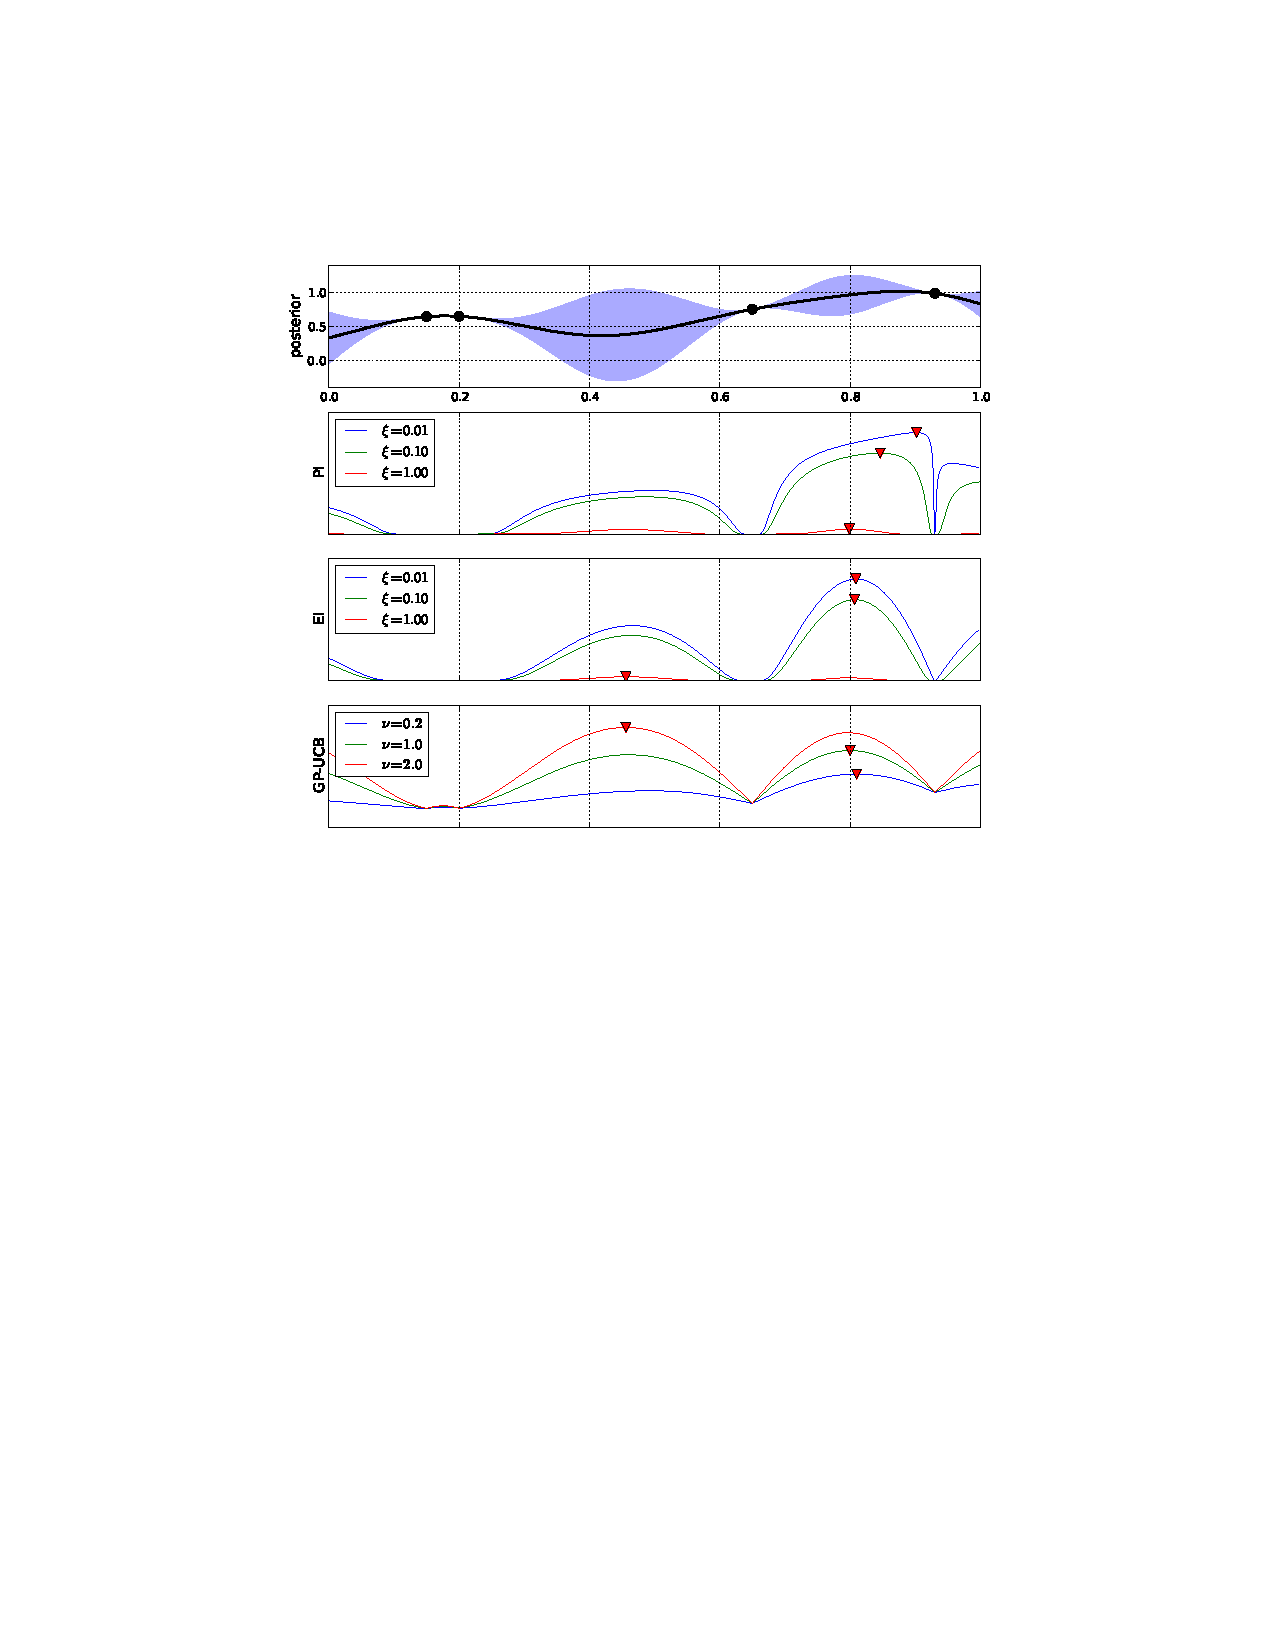
\includegraphics[width=0.8\textwidth]{figures/bayopt_acqui.pdf}
\caption{The figures demonstrate examples of acquisition functions in different settings. The black points indicate the observations. The red triangles indicate the maximum of the acquisition functions. The $\xi$ and $\nu$ are the hyperparameters that have a similar effect of the exploration ratio, where a higher value means choosing exploring more \cite{brochu2010tutorial}.}
\label{bayesian optimization2}
\end{figure}

The time for evaluating the objective function can also depend on the value of the hyperparameter. In \textit{Per Second}  method raised in \cite{snoek2012practical}, the Bayesian optimization algorithm maintains a model of the objective function evaluation time $\mu_{s}(\mathbf{x})$ besides the main surrogate model. The acquisition function with this method is calculated with 
\begin{equation}
    \mathrm{EI}_{ps}(\mathbf{x})=\frac{\mathrm{EI}(\mathbf{x})}{\mu_{s}(\mathbf{x})}.
\end{equation}



\FloatBarrier

\section{Classification Algorithms: Support Vector Machine}

Statistical classification is a supervised learning problem of training a model categorizing new, unlabeled data based upon its relevance to known, labeled data. From the results of the classifiers we can also obtain the decision boundary of the data, which can be used for the determination of the range of the hyperparameters in our implementation. There are a large number of classification methods, such as logistic regression, support vector machines, k-nearest neighbors and neural networks.

\subsection{Basics of the Support Vector Machines}

Support vector machines (SVM) are a set of supervised learning methods used for classification, regression and outliers detection \cite{suykens1999least}. The support vector machines are trained with training examples labeled with different categories. A trained SVM can show the classification boundary between categories and classify unknown examples into a category.

The basic idea of SVM is to find a hypersurface splitting different categories that maximize the distance from data points to the hypersurface. Classifiers with this hypersurface can minimize the risk of the classification \cite{vapnik1999overview}. In a typical binary classification problem, the training set is given as $N$ data points $\{x_{i},y_{i}\}^{N}_{i=1}$, where $x_{i} \in \mathbb{R}^n$ is the $i$th input pattern and $y_{i} \in \mathbb{R}$ is the $i$th output pattern. A linear support vector machine constructs a classifier of the form
\begin{equation}
f(x)=\mathrm{sign}( w^\top x +b).
\end{equation}

To ensure the robustness of the classification, the distance between data points and classification hypersurface should be higher than a margin. For simplicity, the margin is often set at 1, which can be presented as
\begin{equation}
y_{i}(w^\top x_{i}+b)\geqslant 1.
\end{equation}


In case the separation hypersurface is not existed, some of the data points are allowed to locate more close to the hypersurface or even locate at the other side of the plane. Therefore, a slack variable $\xi_{i}$ is introduced, and the constraints for the classifier can be represented as
\begin{equation}
y_{i}(w^\top x_{i}+b)\geqslant 1 - \xi_{i},
\end{equation}
\begin{equation}
\xi_{i}\geqslant 0.
\end{equation}

The distance between the data points and the hypersurface can be represented as $\frac{y_{i}(w^\top x_{i}+b)}{\left \| w \right \|}$. Moreover, the summation of the slack variables $\xi_{i}$ should be minimized, the objective function can be represented according to \cite{suykens1999least} as 

\begin{equation}
L(w, \xi_{i})=\frac{1}{2}\left \| w^{2} \right \|+c\sum_{i=1}^{N} \xi_{i}.
\label{regularization svm}
\end{equation}
Here $c$ is a parameter determines the trade-off between increasing the margin size and ensuring that the ${\vec {x}}_{i}$ lie on the correct side of the margin.

\subsection{Nonlinear Kernels}

In order to deal with the nonlinear classification problems, nonlinear transition functions are introduced to replace the dot product kernel function in the linear SVM. The transition function maps the input space into a higher dimensional space. The new classifier with a nonlinear transition function $\phi(\cdot )$ can be represented as

\begin{equation}
f(x)=\mathrm{sign}( w^\top \phi(x) +b).
\end{equation}

The kernel function can represent the transition function implicitly. Then the SVM is able to be trained in that feature space and have the nonlinearity without explicit computation of the transition function. A general kernel $k$ has the relationship with the transition function as follows

\begin{equation}
k(\mathbf{x}, \mathbf{x'}) =\frac{\| \phi(\mathbf{x}) \|^2+\| \phi(\mathbf{x'}) \|^2-d(\phi(\mathbf{x'}),\phi(\mathbf{x'}))^2}{2}.
\end{equation}

One of the most widely used kernel function is the Gaussian radial basis function (RBF) kernel \cite{vert2004primer}

\begin{equation}
k_{g}(\mathbf{x}, \mathbf{x'}) = \exp\left(-\frac{\|\mathbf{x} - \mathbf{x'}\|^2}{2\sigma^2}\right).
\end{equation}
The Gaussian kernel will be used in the following part of the thesis.


\section{Overfitting and Remedy}

% \textcolor{red}{new section}

In machine learning problems including regression and classification, overfitting means the trained model fits so exactly to the training dataset, that fails to predict future observations in more general cases. This problem often happens when the prediction model in training is much more complex than the model of the dataset, or the training dataset is not large enough to show the general characteristic of the whole dataset that we are interested in. In this case, the model learns not only the information but also the noise in the training data, and a high accuracy on the training data does not imply a high accuracy on the whole data. To overcome overfitting, many methods have been introduced into the machine learning area, such as regularization, cross-validation, early stopping, or dropout.

\begin{figure}[htb]
\centering
\begin{subfigure}[t]{0.4\textwidth}
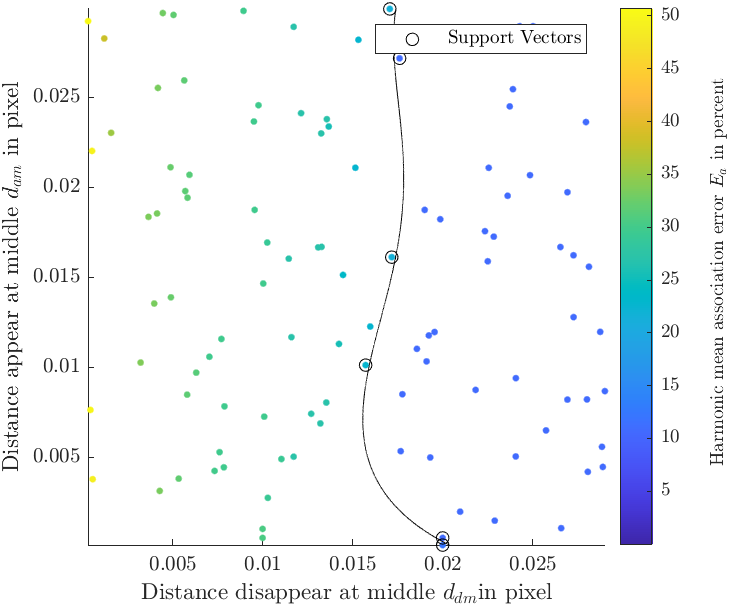
\includegraphics[width=\textwidth]{figures/Asso/overfitting2.png}
\caption{An SVM classification without overfitting. The kernel size is set as 0.5.}
\end{subfigure}
% \hfill
\quad
\begin{subfigure}[t]{0.4\textwidth}
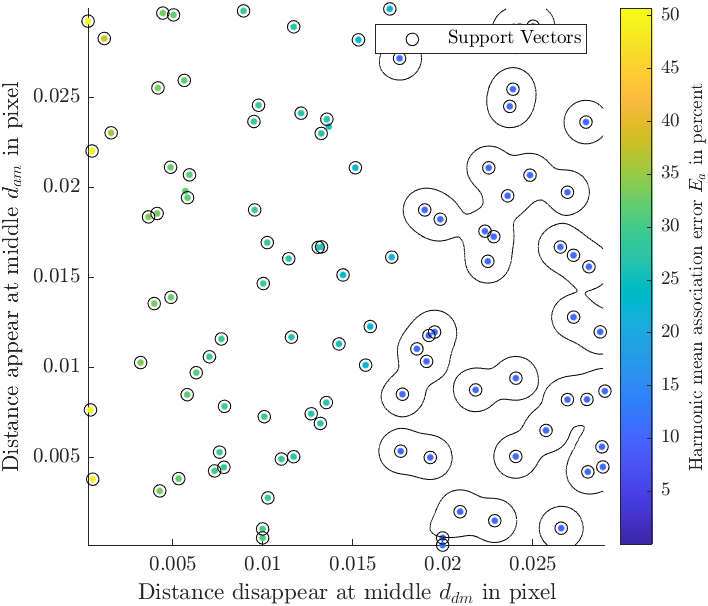
\includegraphics[width=\textwidth]{figures/Asso/overfitting1.png}
\caption{An SVM classification with overfitting. The kernel size is set as 0.01.}
\label{overfitting example}
\end{subfigure}
\caption{Overfitting in the SVM. In Figure (b) the robust area is limited only around the training points, which leaves all the other area as unrobust area.}
% \label{overfitting}
\end{figure}

\subsection{Regularization}

Many loss functions only evaluate how the prediction model from training fits the data, but complexity of the prediction model is ignored. Therefore, the prediction model can be severely affected by the noise of each single training data point and have many unnecessary complexity, such as a highly curved decision boundary in classification problem or a polynomial regression model with high degree terms. Regularization brings the model information into the loss function so that the model can keep as simple as possible and eliminate the misleading effect from the high-frequency noise in the training data. In the typical regularization method, a regularization term is added into the loss function to apply a penalty on the complexity of the prediction model $f$ , as
\begin{equation}
L(f,y)=\sum_{i=1}^{n}V(f(x_{i}),y_{i})+\lambda R(f),
\end{equation}
where $V$ is the original loss function and $R$ is a function that presents the complexity of $f$ \cite{poggio1985computational}. 

The regularization method was first raised in the linear regression problem. A linear model $f(\underline{x})=\underline{\omega}^\top \underline{x}$ is characterized with the vector $\underline{\omega}$. In order to minimize the complexity of the model, the $L_{1}$ and $L_{2}$ regularization, which take the 1-norm and 2-norm of $\underline{\omega}$ as the regularization term, are used \cite{ng2004feature}. The $L_{1}$ and $L_{2}$ regularization is expressed with following equations
\begin{equation}
L_{1}(f,y)=\sum_{i=1}^{n}V(f(x_{i}),y_{i})+\lambda \sum_{j=1}^{m} \left| \omega_{j}\right|
\end{equation}
\begin{equation}
L_{2}(f,y)=\sum_{i=1}^{n}V(f(x_{i}),y_{i})+\lambda \sum_{j=1}^{m}\omega_{j}^2
\end{equation}

In SVM, the first term $\frac{1}{2}\left \| w^{2} \right \|$ in the loss function in Equation \Eq{regularization svm} can serve as a regularization term. Therefore, no additional regularization terms are needed. The parameter $c$ can control the importance of the regularization term, where a higher $c$ means the classifier is more regularized \cite{evgeniou2000regularization}. 

In SVMs with Gaussian kernel, selecting the suitable kernel size $\sigma$ can also reduce the chance of overfitting. A higher kernel size means the range of influence of each support vectors is larger, and the number of support vectors is less. As a result, choosing a higher kernel size can help to avoid overfitting. Figure \ref{overfitting rbf} shows the effect of the regularization parameters $c$ and $\sigma$ on the shape of the classification boundary.

\begin{figure}[htb]
\centering
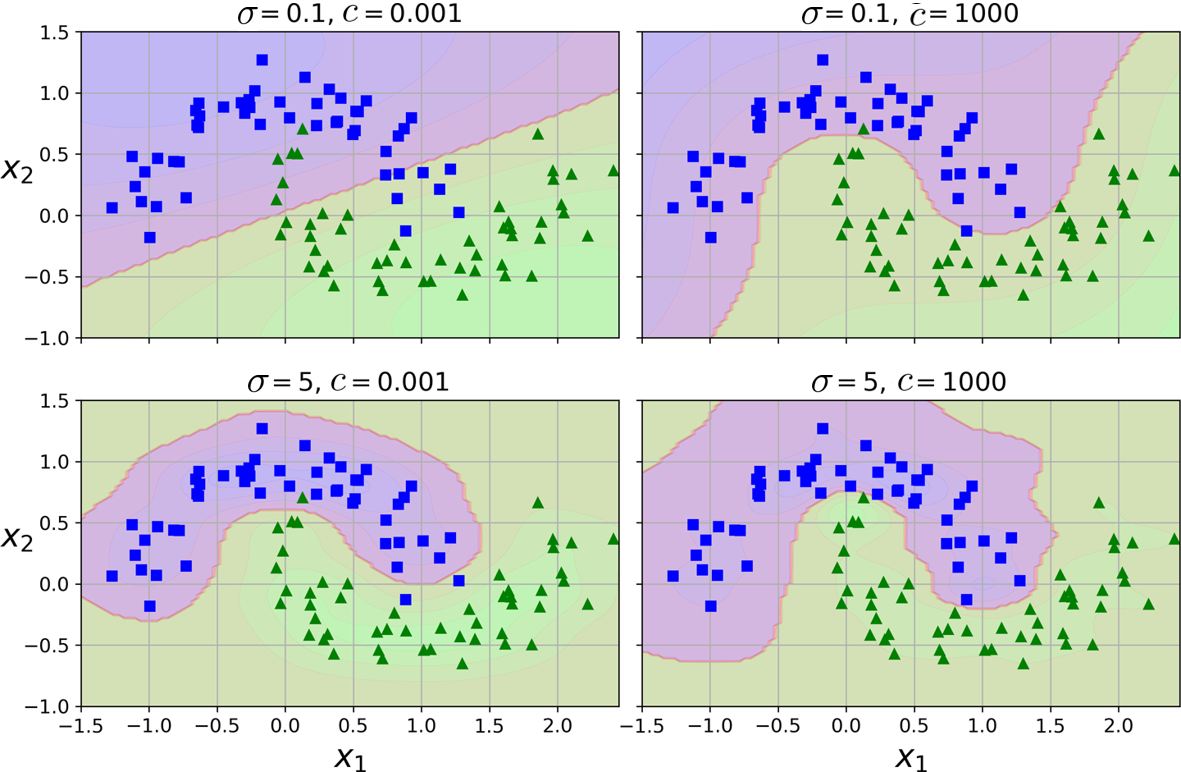
\includegraphics[width=0.8\textwidth]{figures/mls2_0509.png}
\caption{SVM classifiers with an RBF kernel using different regularization parameters \cite{geron2019hands}.}
\label{overfitting rbf}
\end{figure}

\subsection{Cross-Validation}

% \textcolor{red}{I think I mentioned the train-test split in the first paragraph. Is it too short or not clear?}

In order to examine how the trained model fits in the whole dataset, an easy method is the cross-validation. The whole dataset is separated into two sub-datasets: training dataset and test dataset. The prediction model is first trained with the training dataset, and then test the accuracy of the trained model with the test dataset. If the accuracy with the test dataset is also acceptable, the prediction model can be recognized as not overfitting.

However, the amount of data is usually limited. Therefore, it is a waste to use a part of data only for testing and leave the information contained in these data unused in training. The selection of test datasets can also have a great influence on model performance \cite{james2013introduction}. To reduce these effects, the cross-validation is preformed multiple rounds with different divisions, and the validation results from all rounds are combined for estimation of the general model performance.

K-fold cross-validation randomly splits the whole dataset into $k$ groups, or folds, of approximately equal size. In each training, a group is left out as the validation dataset, and the other $k-1$ groups are used as the training data. After doing $k$ times of training, we get $k$ model trained with different data. The final trained model takes the best fit model or the average of all models. With the $k$ times of training, all the information in the datasets can be learned by the prediction model, and the influence of the selection of the test dataset is minimized.

The most widely used $k$ value is 10, 5 and 1. When $k=1$, the method is also called leave-one-out cross-validation. Increasing $k$ increases the accuracy of training, but also increases the computational demand. There are also literatures reporting that the performance with $k=10$ is better than the leave-one-out cross-validation \cite{james2013introduction}.








